\documentclass[12pt,fleqn]{article}
\setlength{\parindent}{0pt}
\usepackage{graphicx}
\usepackage{listings}
\usepackage[latin5]{inputenc}
\setlength{\parskip}{8pt}
\setlength{\parsep}{0pt}
\setlength{\headsep}{0pt}
\setlength{\topskip}{0pt}
\setlength{\topmargin}{0pt}
\setlength{\topsep}{0pt}
\setlength{\partopsep}{0pt}
\setlength{\mathindent}{0cm}

\begin{document}
MIT OCW Cok Degiskenli Calculus - Ders 3

Capraz carpimlar hakkinda bilinmesi gereken bazi sasirtici gelebilecek
kurallar var. Bunlardan bir tanesi $\vec{A} \times \vec{B} \ne \vec{B}
\times \vec{A}$. Niye boyle? Bunu 
gormenin yollarindan bir tanesi geometrik olarak dusunmek. Sag el kuralini
dusunursek, yonun niye farkli olabilecegini anlariz. Isaretler tam terstir, yani

\[  \vec{A} \times \vec{B} = - \vec{B}\times \vec{A} \]

Determinant acilimini da dusunursek, ikinci terim eksi isareti tasir, ama
carpim sirasi degisince eksi isaretinin yeri degisir. 

Peki $\vec{A} \times \vec{A}$ nedir? Capraz carpim alan hesabinda onemli
olduguna gore ve $\vec{A} \times \vec{A}$'in bir parallelogram
yaratmayacagina gore (ya da sifir alanli bir parallelogram yaratacagina
gore) cevap sifir, daha dogrusu sifir ``vektoru'' (o vektorun buyuklugu de
tabii ki sifir).

Uygulamalar

Diyelim ki bize uzayda 3 nokta verildi, ve bu noktalari iceren bir duzlemin
formulunu bulmamiz gerekiyor. 3 nokta 3 boyutlu uzayda bir duzlem yaratmak
icin yeterli, bunu biliyoruz. Bunun icin bir dorduncu nokta $P$ hayal
edelim ki bu noktanin ogeler $x,y,z$ olsun.

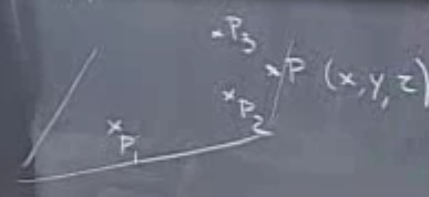
\includegraphics[height=2cm]{3_1.png}

Simdi duzlemi tanimlayalim. Su sekilde 3 tane vektor yaratalim

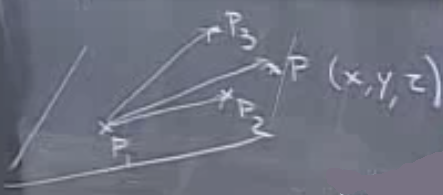
\includegraphics[height=2cm]{3_2.png}

Bu vektorlerin ayni duzlem uzerinde olmasi, ayni zamanda bu vektorlerin
tanimladigi parallelipipe'nin hacimsiz olmasi demektir. Yani birisi
uzerinden bastirip onu dumduz etmistir sanki, sadece alani kalmistir. 

Bunu formulsel olarak soylemenin yolu sudur:

\[ det(\vec{P_1P},\vec{P_2P},\vec{P_3P}) = 0 \]

Gercek uygulama baglaminda problem bize $P_1,P_2,P_3$ sayilarini vermis
olacakti bu sayilari ustteki formule yerlestirirdik, tanimsiz olan sadece
$x,y,z$ kalirdi, ve bu $x,y,z$'ler ile beraber elde edilecek formul bu
noktalarin tanimladigi alan olurdu.

Bu hesabi daha da hizli yapmanin bir yolu var. Alttaki resmi dusunelim. 

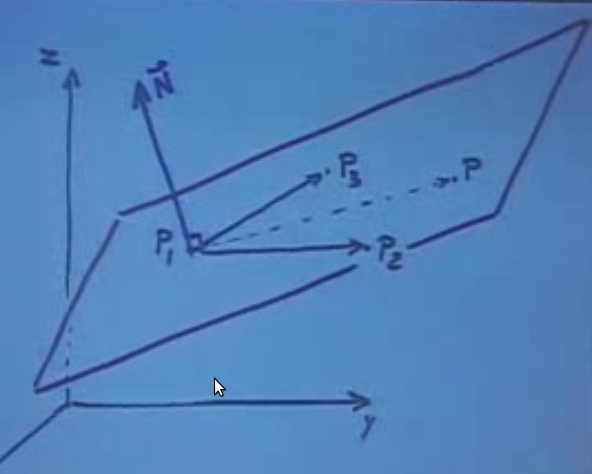
\includegraphics[height=4cm]{3_3.png}

Resme bakalim. Duzlem uzerindeki iki vektore dik bir $\vec{N}$'i nasil
hesaplayacagimizi biliyoruz (carpraz carpim ile). Devam edelim, $x,y,z$
degiskenlerini iceren ucuncu bir vektor $\vec{P_1P}$'in ayni duzlemde
olmasi demek, bu $\vec{N}$ vektorune dik olmasi demektir ($\vec{N}$
``normal vektor'' olarak isimlendirilir). Bunu matematiksel olarak nasil
ifade ederiz? Dikligin formulsel karsiligini biliyoruz, noktasal carpim
sifir olmali.

\[ \vec{P_1P} \cdot \vec{N} = 0 \]

$\vec{N}$ hesabi icin 

\[ \vec{N} = \vec{P_1P_2} \times \vec{P_1P_3}\]

Bu kadar. 

Ek not, eger capraz carpimin sirasini degistirmis olsaydim, o zaman ustteki
hesabin ters yonunde bir baska dik vektor elde ederdim, duzlem yine ayni
olurdu, sadece baska bir normal vektor olurdu. Bu problem degil, herhangi
bir duzlemin sonsuz sayida normal vektoru olabilir. Elde ettigimiz bir
normal vektoru herhangi bir sabit ile carpinca yeni bir normal vektor elde
etmis olurdum cunku. 

\[ \vec{P_1P} \cdot \vec{N} = 
\vec{P_1P} \cdot (\vec{P_1P_2} \times \vec{P_1P_3})
\]

Esitligin sagindaki carpima uclu carpim (triple product) deniyor. 

Son formulu takip edersek determinant sifirligi uzerinden tanimlanan diger
formul ile ayni sonucu getirdigini gorurduk. 

Matrisler

$A \ B$ seklindeki bir matris carpiminda hangi hucrenin hangi kolon, hangi
satirin noktasal carpim sonucu (answer) oldugunu hayal edebilmek icin
alttaki sekil faydali olabilir. $B$, sonuc matrisinin (altta bos) ustunde
hayal edilir, ve carpi isaretindeki sonuc icin onun heme ustundeki kolona,
ve hemen yanindaki satira gidilir.

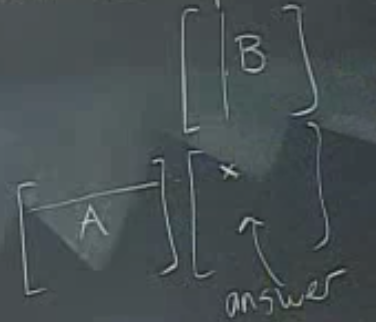
\includegraphics[height=4cm]{3_4.png}

Sezgisel (intuitive) olarak $AB$ carpimi neyi temsil eder? Bu carpimi soyle
dusunebiliriz, once $B$ transformu yap, sonra $A$ transformu yap. Bu biraz
acaip gelebilir, cunku normalde islemleri soldan saga yapmaya
alisigizdir. Fakat $AB$'yi belki de sirali fonksiyon islemleri olarak
gormek daha dogru olur, mesela $f(g(x))$ gibi. Burada once $g$ uygulanir,
sonra $f$ uygulanir. 

\[ (AB)X = A(BX) \]

Ustteki aktarim kanunudur (associativity) ve ``iyi davranan'' carpimlarin
bir ozelligidir. Bu arada ustteki carpimin noktasal degil, matris carpimi
olduguna dikkat edelim. 

Not: $AB \ne BA$. En azindan sagdaki carpimin olabilecegini beklemememiz
gerekir. $AB$ carpimi boyutlar uydugu icin mumkun olmustur, fakat bu uyumlu
boyutlar yerler degisince belki mumkun olmaz. Boyutlar olsa bile sonuc
farkli cikabilir, o sebeble esitlik farz edilemez. Ufak bir Python kodu ile
test edelim:

\lstinputlisting[language=Python]{dot.py}

Sonuclar farkli cikacak. 

Ornek

Cevirmek / Rotasyon

Bir duzlem uzerinde bir vektoru $90^o$, saat yonu tersine cevirmek icin 

\[ R =
\left[\begin{array}{rr}
0 & -1 \\
1 & 0
\end{array}\right]
 \]

Ilginc bir durum

\[ R^2 =
\left[\begin{array}{rr}
-1 & 0 \\
0 & -1
\end{array}\right]
 \]

Yani birim (identity) matrisinin negatifi. Niye boyle oldu? Dusunelim, eger
bir vektoru 90 derece dondurursem, sonra bir daha 90 derece dondurursem, o
zaman tam tersi yone gitmis olurum. Birim matrisin negatifi de budur
zaten. 


\end{document}
